\chapter{Descripción del Trabajo}
\label{cap:descripcionTrabajo}

En los capítulos anteriores se ha presentado una visión general del proyecto y se han descrito las herramientas principales empleadas, así como las alternativas consideradas durante su desarrollo. En este capítulo se expone de forma detallada el trabajo realizado, describiendo cada una de las fases del pipeline y las decisiones técnicas que se fueron adoptando a lo largo del proceso.

Antes de entrar en cada etapa, resulta útil mostrar un frame del vídeo original, es decir, la entrada del sistema antes de aplicar cualquier tipo de procesamiento.

\begin{figure}[H]
    \centering
    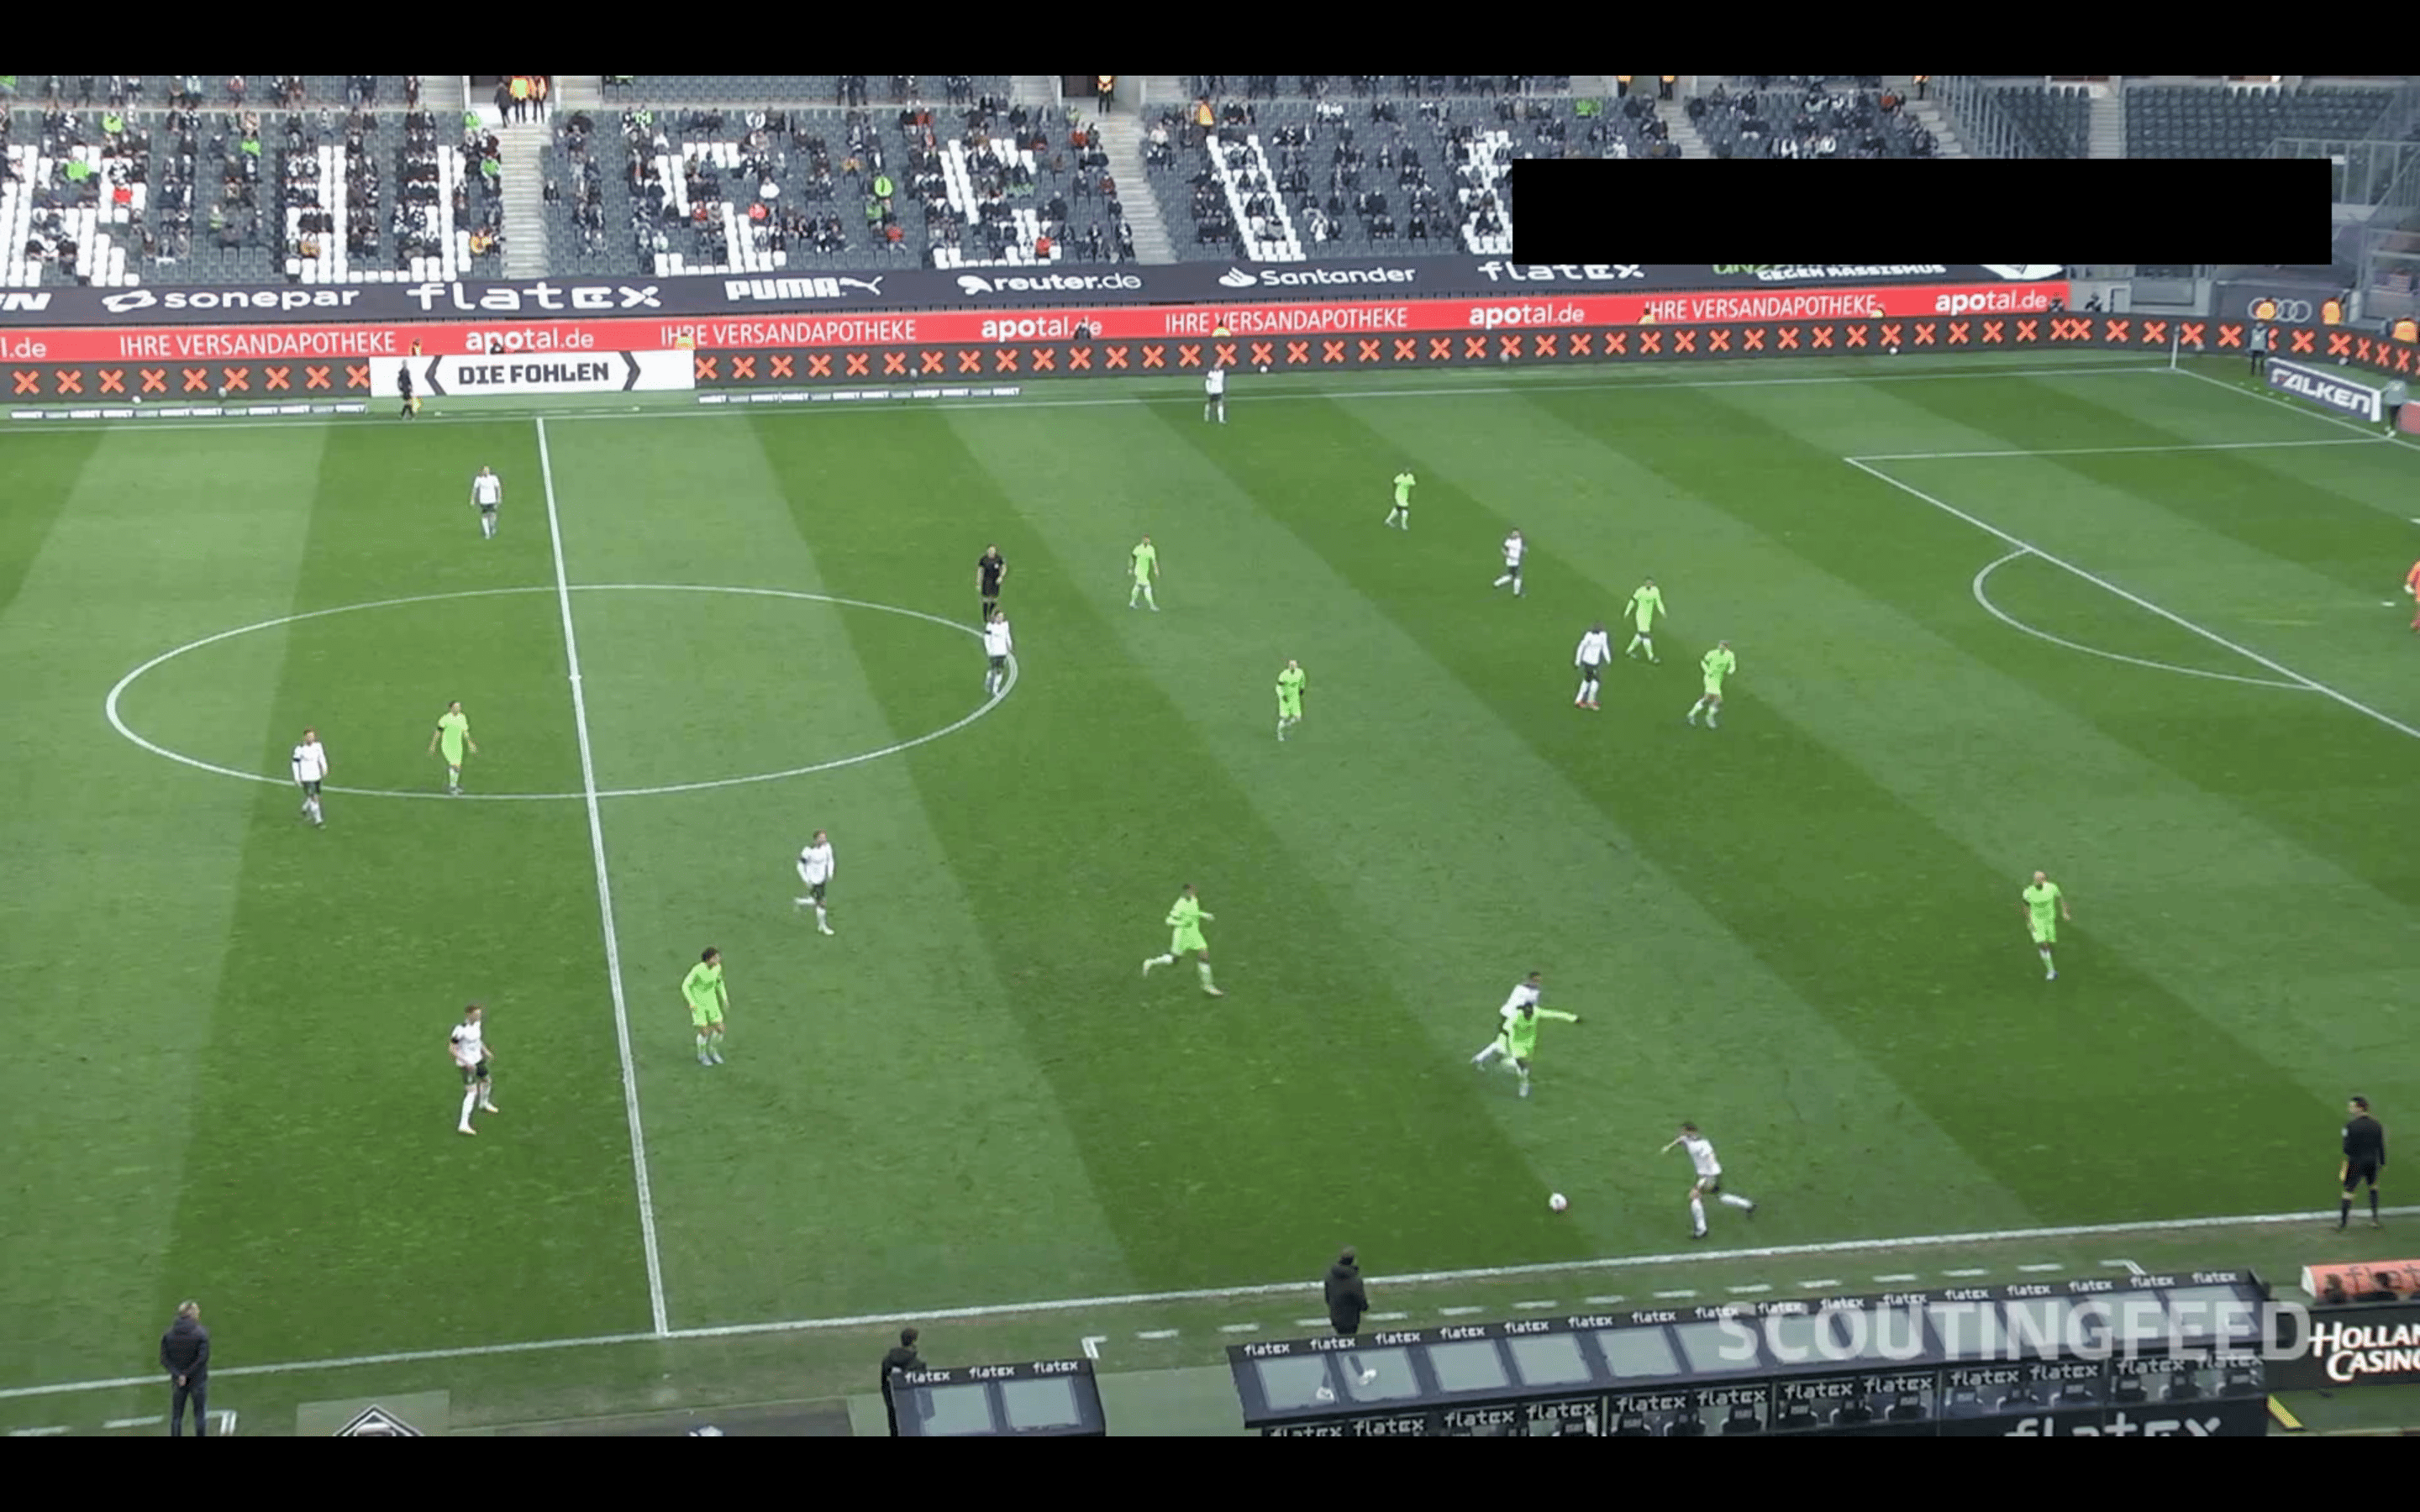
\includegraphics[width=0.9\textwidth]{Imagenes/Propias/Raw_image.png}
    \caption{Frame original del vídeo de entrada.}
    \label{fig:raw-football-image}
\end{figure}




%\section{Interfaz}

La interfaz se ha dejado para el final porque actúa como punto de unión entre varias partes del sistema. No realiza por sí sola la detección, el tracking, la identificación de jugadores o la generación de audio, pero sí permite configurar una ejecución completa y lanzar los procesos necesarios de forma coordinada.

\begin{figure}[H]
\centering
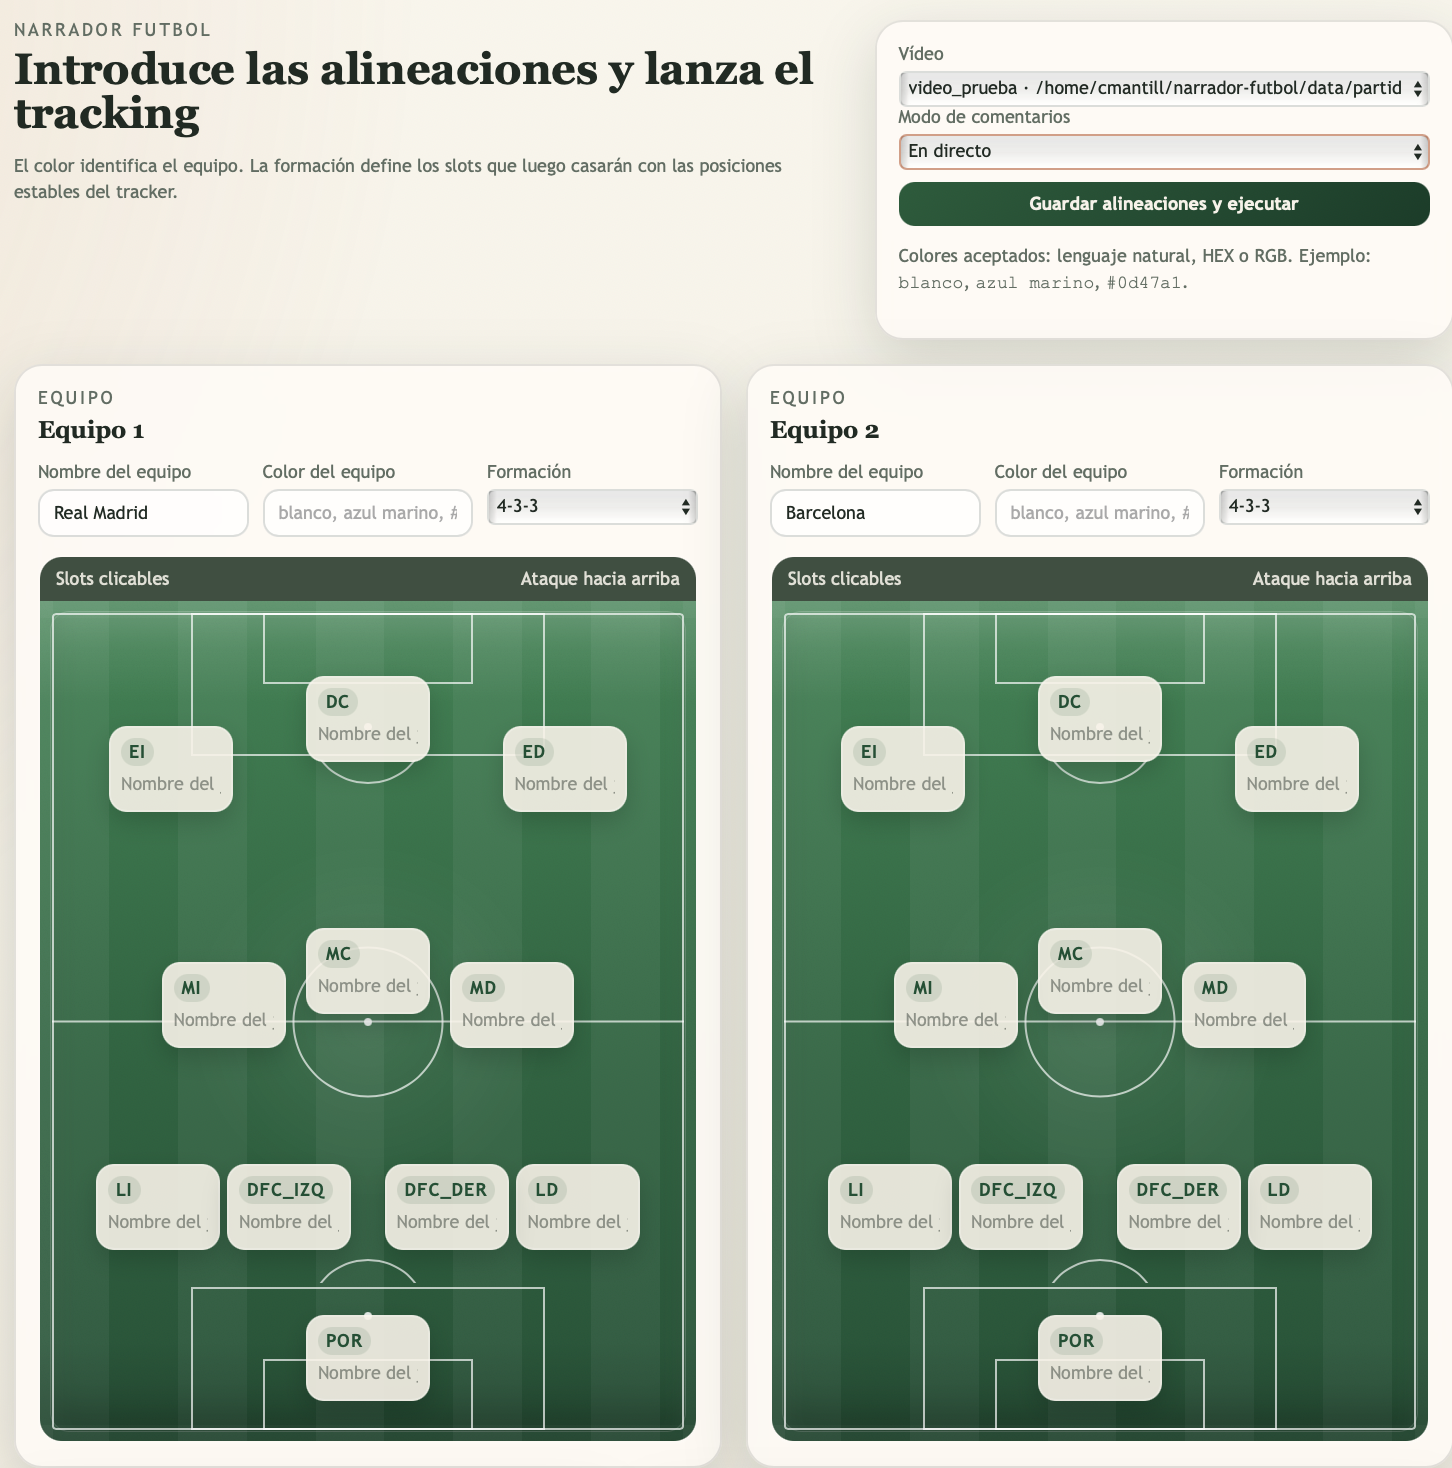
\includegraphics[width=0.9\linewidth]{Imagenes//Propias//interfaz.png}
\caption{Interfaz web de la aplicación.}
\label{fig:interfaz}
\end{figure}

La \hyperref[fig:interfaz]{Figura~\ref*{fig:interfaz}} muestra la interfaz web de la aplicación. Esta cumple dos funciones principales. Por un lado, recoge información que no puede deducirse de forma fiable únicamente a partir del vídeo, como el nombre de los equipos y su asociación al color, las formaciones y los nombres de los jugadores. Por otro lado, actúa como disparador del pipeline completo: guarda la configuración introducida, lanza el tracking, activa el sistema de comentarios y muestra el estado de la ejecución.

\subsection{Arranque de la aplicación}

Al iniciar la aplicación se levanta un servidor web local que sirve la interfaz. En paralelo, también se prepara el sistema de comentarios. Por defecto, la aplicación intenta utilizar un backend local basado en \texttt{llama.cpp} si existe configuración disponible; si no, puede recurrir a Ollama. Además, se inicializa el backend de voz configurado, que por defecto es XTTS, aunque también puede utilizar ElevenLabs si se lanza la aplicación con esa opción.

Una característica importante es el precalentado del comentario de introducción. Este comentario se genera en segundo plano al abrir la interfaz, antes de que el usuario haya terminado de rellenar todos los campos. La finalidad es reducir la espera al lanzar una ejecución, ya que el comentario de introducción suele ser más largo y su síntesis puede tardar más que la de una acción breve. 

\subsection{Bloqueo inicial del formulario}

La primera información que debe introducir el usuario es el nombre de los dos equipos. Hasta que ambos nombres están completos, la interfaz mantiene bloqueados el selector de vídeo, el modo de comentarios, los colores, las formaciones y los campos de jugadores.

Esta restricción evita lanzar ejecuciones incompletas y garantiza que los datos básicos del partido estén disponibles antes de construir la especificación de alineaciones. Además, la interfaz está diseñada para no reconstruir las tarjetas de equipo mientras se está escribiendo, evitando pérdidas de foco o interrupciones durante la edición.

\subsection{Selección del vídeo}

Como el proyecto trabaja con vídeos ya grabados, la interfaz permite seleccionar el vídeo que se va a procesar. El selector se alimenta de los vídeos definidos en la configuración del proyecto, mostrando las claves disponibles y sus rutas asociadas.

Al lanzar la ejecución, ese vídeo se pasa al pipeline de tracking. El resultado final se muestra después dentro de la propia interfaz mediante un reproductor HTML, de forma que el usuario puede revisar el vídeo procesado sin tener que buscar manualmente el archivo generado.

\subsection{Formaciones y alineaciones}

La interfaz permite seleccionar una formación para cada equipo. Las formaciones soportadas son:

\begin{itemize}
    \item \texttt{4-3-3}
    \item \texttt{5-3-2}
    \item \texttt{4-4-2}
\end{itemize}

Cada formación define un conjunto de slots visibles para el usuario y una correspondencia interna con los roles que consume el sistema de tracking. Por ejemplo, en una formación con dos 4 defensas pueden aparecer slots diferenciados como \texttt{LI} y \texttt{LD}.

La interfaz dibuja los slots sobre un campo de fútbol, con la orientación de ataque hacia arriba. El usuario introduce el nombre de cada jugador en el slot correspondiente. Esta información se guarda después en una especificación de alineaciones que será utilizada por el módulo de identificación posicional.

Durante el tracking, el sistema estima el rol estable de cada jugador. Cuando un track ya tiene equipo y rol suficientemente estabilizados, se utiliza la alineación introducida para asociar ese track con el nombre real del jugador. De esta forma, los comentarios pueden mencionar jugadores concretos en lugar de referirse únicamente a identificadores internos.

\subsection{Colores de los equipos}

Otro dato necesario es el color de camiseta de cada equipo. La interfaz acepta colores escritos de tres formas:

\begin{itemize}
    \item nombres comunes, como \texttt{blanco}, \texttt{rojo}, \texttt{azul} o \texttt{negro};
    \item valores HEX, como \texttt{\#ffffff};
    \item valores RGB, como \texttt{255,255,255}.
\end{itemize}

Internamente, los colores introducidos se convierten primero a RGB y después al espacio LAB de OpenCV. Este espacio es más adecuado para comparar colores porque aproxima mejor diferencias perceptuales que el RGB directo.

En la fase de identificación de equipos, el sistema extrae muestras de color de camiseta mediante clustering. Los centroides obtenidos se comparan con los colores de referencia introducidos por el usuario, y cada equipo se asocia al centroide más cercano. Posteriormente, el sistema puede actualizar la referencia con los colores realmente observados en el vídeo, haciendo que la asignación sea más robusta que usar únicamente el valor escrito por el usuario.

\subsection{Modo de comentarios}

La interfaz ofrece dos modos de comentarios: en directo y en diferido. Aunque los vídeos sean grabados, el modo en directo simula una retransmisión: a medida que avanza el procesamiento, el sistema intenta reproducir los comentarios que se van generando.

En modo directo no se reproduce necesariamente todo lo que se genera. Si ya hay un audio sonando, el sistema evita acumular una cola larga de comentarios antiguos. En su lugar, conserva el comentario escrito en el manifiesto y solo reproduce audio cuando el canal está libre. Además, acciones urgentes como tiros o goles pueden interrumpir comentarios contextuales menos importantes.

En modo diferido, los comentarios se generan y se guardan, pero no se reproducen durante el procesamiento. Al terminar, se construye una pista de audio a partir del manifiesto de eventos y se mezcla con el vídeo final. Esta estrategia permite alinear mejor cada comentario con el instante real de la acción, compensando la latencia de generación del audio.

\subsection{Estado, logs y resultados}

La interfaz muestra el estado de la ejecución en tiempo real. Para cada run se guarda un identificador reconocible que incluye fecha, equipos, vídeo y un sufijo corto. También se guarda el estado actual, el log del tracking, la especificación de alineaciones y el manifiesto de comentarios.

En la pantalla principal se muestran:

\begin{itemize}
    \item estado de la ejecución;
    \item equipos seleccionados;
    \item vídeo procesado;
    \item ruta de salida;
    \item estado del comentario de introducción;
    \item estado del ensamblado de audio;
    \item últimas líneas del log del tracking;
    \item vídeo final cuando está disponible.
\end{itemize}

El servidor de la interfaz también soporta peticiones parciales de archivo, lo que permite que el vídeo final se pueda reproducir correctamente en el navegador mediante streaming progresivo.

\subsection{Vídeo final}

Al terminar el tracking, la interfaz intenta ensamblar la pista de comentarios con el vídeo final. El resultado se reexporta en un formato compatible con navegadores modernos, usando H.264/AAC y limitando la resolución si es necesario. Esto evita problemas habituales de reproducción, como vídeos generados con códecs no soportados por el navegador o archivos demasiado pesados.

De esta forma, la interfaz no solo lanza el procesamiento, sino que también permite revisar el resultado final desde la misma página.


% \section{Resumen de procesos y tiempos en GPU}
% \input{Capitulos/04_Descripcion_del_Trabajo/410_Demo_final}